\documentclass[a4paper,10pt]{article}
\usepackage[utf8]{inputenc}
\usepackage{amsmath}
\usepackage{fullpage}
\usepackage{hyperref}
\usepackage{graphicx}
\usepackage{listings}
\usepackage{color}

\definecolor{mygreen}{rgb}{0,0.6,0}
\definecolor{mygray}{rgb}{0.5,0.5,0.5}
\definecolor{mymauve}{rgb}{0.58,0,0.82}

\lstset{ 
  backgroundcolor=\color{white},   % choose the background color; you must add \usepackage{color} or \usepackage{xcolor}; should come as last argument
  basicstyle=\footnotesize,        % the size of the fonts that are used for the code
  breakatwhitespace=false,         % sets if automatic breaks should only happen at whitespace
  breaklines=true,                 % sets automatic line breaking
  captionpos=b,                    % sets the caption-position to bottom
  commentstyle=\color{mygreen},    % comment style
  deletekeywords={...},            % if you want to delete keywords from the given language
  escapeinside={\%*}{*)},          % if you want to add LaTeX within your code
  extendedchars=true,              % lets you use non-ASCII characters; for 8-bits encodings only, does not work with UTF-8
  firstnumber=1,                   % start line enumeration with line 1000
  frame=single,	                   % adds a frame around the code
  keepspaces=true,                 % keeps spaces in text, useful for keeping indentation of code (possibly needs columns=flexible)
  keywordstyle=\color{blue},       % keyword style
  language=Python,                 % the language of the code
  morekeywords={*,...},            % if you want to add more keywords to the set
  numbers=left,                    % where to put the line-numbers; possible values are (none, left, right)
  numbersep=5pt,                   % how far the line-numbers are from the code
  numberstyle=\tiny\color{mygray}, % the style that is used for the line-numbers
  rulecolor=\color{black},         % if not set, the frame-color may be changed on line-breaks within not-black text (e.g. comments (green here))
  showspaces=false,                % show spaces everywhere adding particular underscores; it overrides 'showstringspaces'
  showstringspaces=false,          % underline spaces within strings only
  showtabs=false,                  % show tabs within strings adding particular underscores
  stepnumber=1,                    % the step between two line-numbers. If it's 1, each line will be numbered
  stringstyle=\color{mymauve},     % string literal style
  tabsize=4,	                   % sets default tabsize to 2 spaces
  title=\lstname                   % show the filename of files included with \lstinputlisting; also try caption instead of title
}


%opening
\title{NUR Assignment 2}
\author{Christiaan van Buchem - s1587064}

\begin{document}

\maketitle

\begin{abstract}
 In this document I will be giving my answers to the questions of the second assignment for the Numerical Recipes for Astrophysics course. For each question I will give a short introduction, write out any non-coded answers that may be required, produce the print statements and the plots, and finally I will show the script used to produce the results.  
\end{abstract}

\section{Normally distributed pseudo-random numbers}

\subsection{RNG}

For exercise 1 we were tasked with writing a random number generator that returns a random floating point number between 0 and 1. At minimum we had to use some combination of an MWC and a 64-bit XOR-shift. The plots made to test the quality of the RNG can be seen in Figures \ref{fig:1a}, \ref{fig:1b}, and \ref{fig:1c}.


\begin{figure}[h!] 
	\begin{center}
    	%
		\subfigure{%
			\label{fig:1a}
			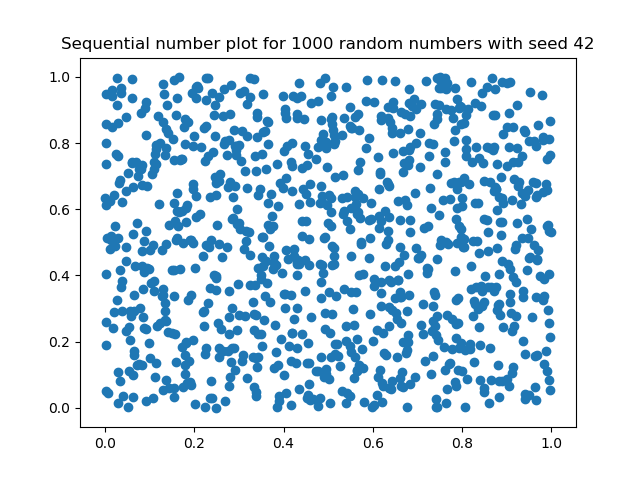
\includegraphics[width=0.45\linewidth]{./plots/1a.png}
		}%
		\subfigure{%
			\label{fig:1b}
			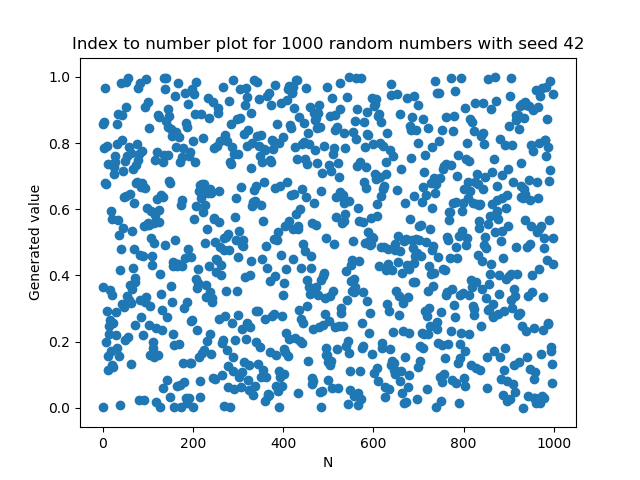
\includegraphics[width=0.45\linewidth]{./plots/1b.png}
		}
	\end{center}
	\captionsetup{width=0.8\linewidth}
	\vspace*{-7mm} %reduce space between caption and figure
	\caption{\textit{Left:} Sequential number plot showing that it appears that each number is independent of its predecessor. \textit{Right:} Index to number plot showing that there does not appear to be a relation between the index of a number and its value.}
	\label{fig:1ab}
\end{figure}

\begin{figure}[h!]
  \centering
  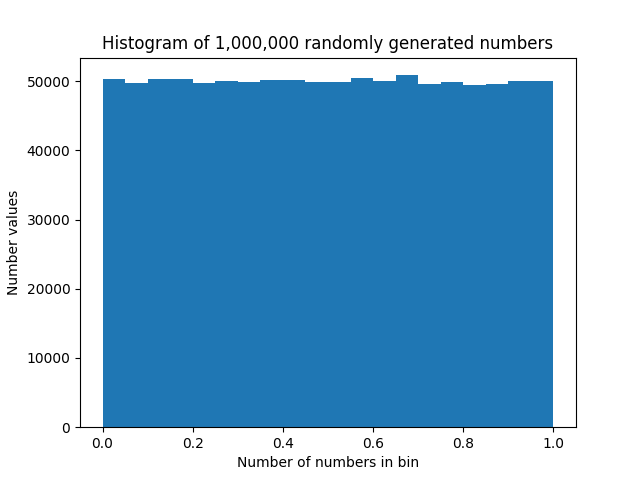
\includegraphics[width=0.8\linewidth]{./plots/1c.png}
  \caption{This histogram places the random number generator under a sharper knife, allowing us to see that there are some fluctuations between the bins. Overal it appears to be quite unbiased.}
  \label{fig:1c}
\end{figure}

\subsection{Box-Muller method}
Using the Box-Muller method we had to generate 1000 normally distributed random numbers. In order to check if they follow the expected distribution we make a histogram with an over-plotted Gaussian. The results can be seen in Figure \ref{fig:1d}.

\begin{figure}[h!]
  \centering
  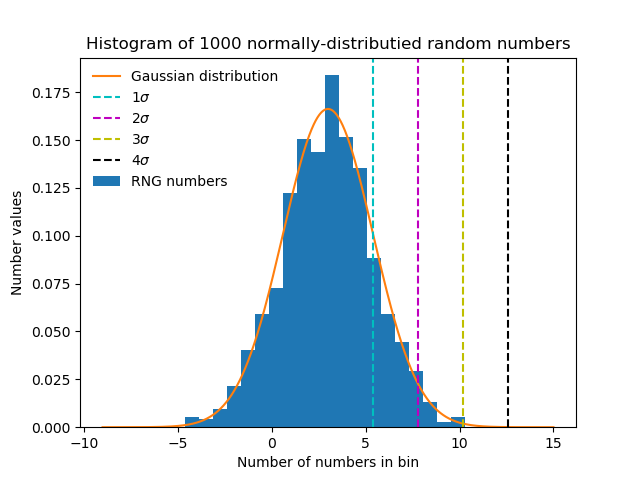
\includegraphics[width=0.8\linewidth]{./plots/1d.png}
  \caption{In this figure we can see that numbers generated using the Box-Muller method do indeed follow the Gaussian distribution.}
  \label{fig:1d}
\end{figure}

\subsection{KS-test}
For this exercise we tested whether or not our function is consistent with the normal distribution. The resulting plot can be seen in Figure \ref{fig:1e}. The slight difference between the two may be attributed to the fact that in the self written KS-test the following approximation was used: 
\[
	P_{KS}(z)\approx
\begin{cases}
	\frac{\sqrt{2\pi}}{z}[(e^{-\pi^2/(8z^2)})+(e^{-\pi^2/(8z^2)})^9+(e^{-\pi^2/(8z^2)})^25],& (z<1.18)\\
	1-2[(e^{-2z^2})-(e^{-2z^2})^4+(e^{-2z^2})^9],	& (z\geq 1.18)
\end{cases}
\]


\begin{figure}[h!]
  \centering
  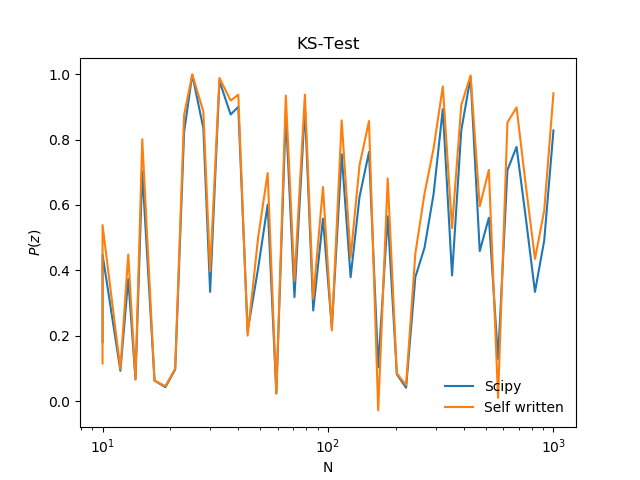
\includegraphics[width=0.8\linewidth]{./plots/1e.png}
  \caption{Here we see that the 'self-written' KS-test follows the Scipy KS-test results almost exactly.}
  \label{fig:1e}
\end{figure}

\subsection{Kuiper's-test}

The same as for the KS-test except that we had to use Kuiper's test. Results can be seen in Figure \ref{fig:1f}.

\begin{figure}[h!]
  \centering
  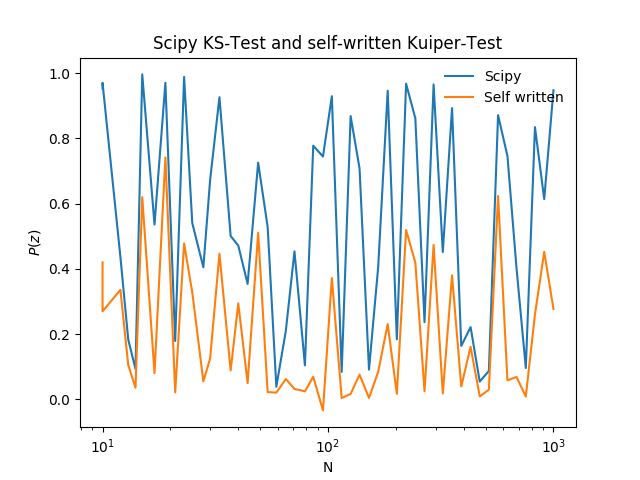
\includegraphics[width=0.8\linewidth]{./plots/1f.png}
  \caption{Here we compare the Kuipers test.}
  \label{fig:1f}
\end{figure}

\subsection{Analysing a dataset}

In this exercise we were tasked with analysing a giving data set using either the KS-test or Kuipers test. The results can be seen in Figure \ref{fig:1g}.

\begin{figure}[h!]
  \centering
  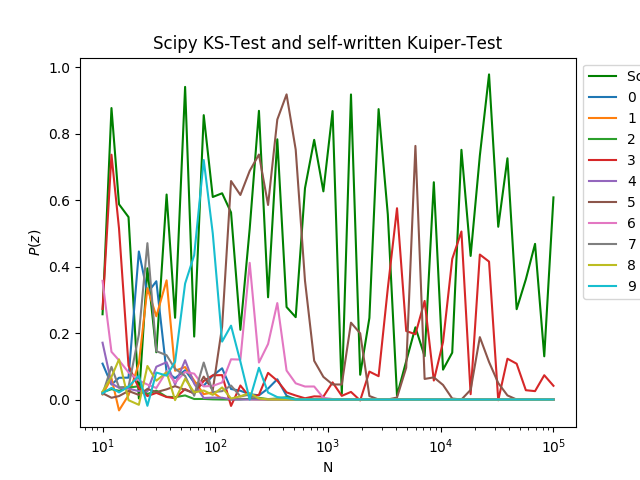
\includegraphics[width=0.8\linewidth]{./plots/1g.png}
  \caption{Analysing the different datasets.}
  \label{fig:1g}
\end{figure}

\subsection{Scripts}

Here we can see the terminal output of the script used for this exercise:
\lstinputlisting{a2_1.txt}

Here is the script used to produce these results: 
\lstinputlisting{a2_1.py}

\section{Making an initial density field}

For this exercise we were asked to generate a Gaussian random field. The field is generated in Fourier Space. The complex Fourier amplitudes are given by $\tilde{Y}=|\tilde{Y}exp(i\phi)$ where $phi$ is a random phase. The power spectrum has the following form: 

\begin{equation}
P(k) \propto k^n
\end{equation}

In Figure \ref{fig:2} the generated Gaussian random fields are given for different n values. 

\color{red}
Choose a minimum physical size and explain how this impacts the maximum physical size, the minimum $k$ and maximum $k$. 

\color{black}

\begin{figure}[h!]
  \centering
  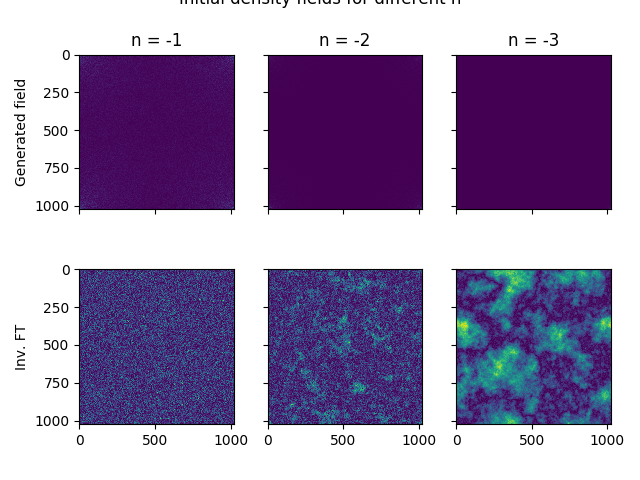
\includegraphics[width=0.8\linewidth]{./plots/2.png}
  \caption{Gaussian random fields for different n values. Notice the clear presence of larger structure when the spectrum is more peaked (lower n).}
  \label{fig:2}
\end{figure}

\subsection{Scripts}

Here we can see the terminal output of the script used for this exercise:
\lstinputlisting{a2_2.txt}

Here is the script used to produce these results: 
\lstinputlisting{a2_2.py}

\section{Linear Structure Growth}

The evolution of density perturbations in the initial universe evolves according to the following equation: 

\begin{equation}
\frac{\partial^2\delta}{\partial t^2} + 2\frac{\dot{a}}{a}\frac{\partial\delta}{\partial t} = \frac{3}{2}\Omega_0H_0^2\frac{\delta}{a^3}
\end{equation}

In the early Universe we can separate the density perturbation as having a spatial part and a temporal part: $\delta = D(t)\Delta(x)$. In the case of a second order equation we have two growth factors. This means that the above partial differential equation becomes: 

\begin{equation}
\frac{d^2D}{d t^2} + 2\frac{\dot{a}}{a}\frac{dD}{dt} = \frac{3}{2}\Omega_0H_0^2\frac{D}{a^3}
\end{equation}

We were asked to look at a Einstein-de Sitter Universe where $\Omega_m = 1$ and the scale factor is given by: 

\begin{equation}
a(t) = (\frac{3}{2}H_0t)^{2/3}
\end{equation}

The density growth equation for this Universe is the following: 

\begin{equation}
\frac{d^2D}{dt^2} = \frac{-4}{3t} \frac{dD}{dt} + \frac{2}{3t^2} D
\end{equation}

For this exercise we were to calculate the numerical solutions for three different sets of initial conditions. These results were then to be compared with the analytical solutions of the ODE. 

In Table \ref{tab:3} we can see the different cases and their analytical solutions. 


\begin{table}[h!]
\begin{center}
\begin{tabular}{c|c|c|c}
 & D(1) & D'(2) & D(t) \\ 
\hline 
case 1 & 3 & 2 & $3t^{2/3}$ \\ 
case 2 & 10 & -10 & $10t^{-1}$ \\ 
case3 & 5 & 0 & $(3t^{5/3}+2)t^{-1}$ \\ 
\end{tabular} 
\label{tab:3}
\caption{The three different sets of initial conditions.}
\end{center}
\end{table}

In Figure \ref{fig:3} we can see the numerical and analytical solutions for the 3 different cases.

\color{red} Mention why they do not match. \color{black}

\begin{figure}[h!]
  \centering
  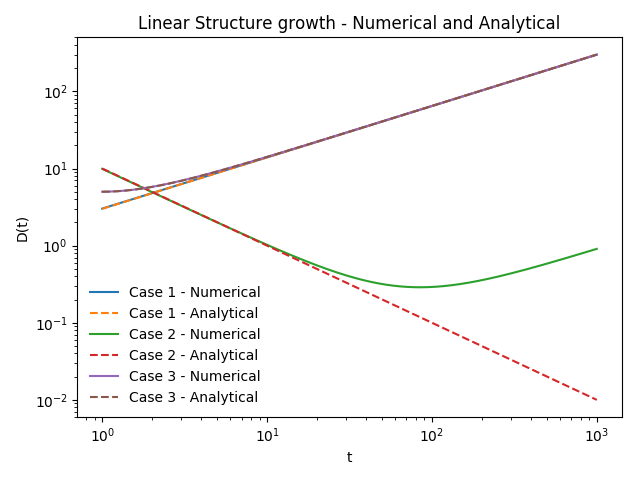
\includegraphics[width=0.8\linewidth]{./plots/3.png}
  \caption{Analytical and numerical solutions to the partial differential equations given in this question.}
  \label{fig:3}
\end{figure}

\subsection{Scripts}

Here we can see the terminal output of the script used for this exercise:
\lstinputlisting{a2_3.txt}

Here is the script used to produce these results: 
\lstinputlisting{a2_3.py}

\section{Zeldovich approximation} 

In this exercise we will be looking at the Zeldovich approximation. 

\subsection{Calculating the linear growth factor to a given redshift.}

Our first task was to integrate the linear growth factor up to a redshift of $z=50$. The integral to be solved is the following:

\begin{equation}
D(z) = \frac{5\Omega_mH_0^2}{2}H(z)\int_z^\infty\frac{1+z'}{H^3(z')}dz'
\end{equation}

Where 

\begin{equation}
H(z)^2 = H^2_0(\Omega_m(1+z)^3+\Omega_\Lambda)
\end{equation}

In order to avoid having to integrate up to $\infty$ we will be substituting $z = \frac{1}{a} -1$. This gives us the following equations:

\begin{equation}
D(a) = \frac{5\Omega_mH_0^2}{2}H(a)\int_0^a\frac{1}{a^3H^3(a')}da'
\end{equation}

Where 

\begin{equation}
H(a)^2 = H^2_0(\frac{\Omega_m}{a^3}+\Omega_\Lambda)
\end{equation}

The resulting value is: $D(1/51) = 0.0196$. The exact number and the way that it was calculated can be found in the print output below. 

\subsection{Calculating the derivative of the linear growth factor at a given redshift}

In order to accomplish this task we had to analytically derive the value of $\dot{D}(t)$. One can calculate this indirectly using the following equation: 

\begin{equation}
\dot{D}(t) = \frac{dD}{da}\dot{a}
\end{equation} 

Where

\begin{equation}
\dot{a} = \frac{H_0}{\sqrt{a}}
\end{equation}


If we use the chain rule we get:

\begin{equation}
\frac{dD}{da} = \frac{5\Omega_mH_0^2}{2}[\frac{dH(a)}{da}I+\frac{dI}{da}H(a)]
\end{equation}

Where

\begin{equation}
I = \int^a_0\frac{1}{a^3H(a)^3}da
\end{equation}


Which gives us: 

\begin{equation}
\dot{D}(a) = \frac{5\Omega_mH_0^3}{2\sqrt{a}}[\frac{-3\Omega_m}{2\sqrt{a^5(\Omega_m+\Omega_\Lambda a^3)}}\int^a_0\frac{1}{a^3H(a)^3}da+\frac{1}{a^3H(a)^3}H_0\sqrt{\frac{\Omega_m}{a^3}+\Omega_\Lambda}]
\end{equation}

The resulting value is: $\dot{D}(1/51) = 1239$ REQUIRE UNITS . The exact number and the way that it was calculated can be found in the print output below. 

\subsection{Evolution of a volume in 2D}

 

\end{document}


 

